\chapter{Introduzione ai metodi Monte Carlo}
\label{sec:monte_carlo}

Avrete sentito tutti in vita vostra la parola \emph{simulazione}---le
simulazioni sono una parte rilevante del lavoro del Fisico, ma cosa
vuol dire esattamente eseguire una simulazione di un sistema fisico su un
calcolatore? In questo capitolo cercheremo di rispondere, sia pur parzialmente,
a questa domanda e di sviluppare i concetti di base rilevanti.


\section{Introduzione: due semplici esempi}

Cominciamo con il primo esempio. Supponiamo di voler stimare numericamente il
valore di $\pi$ con un numero fissato di cifre significative. Storicamente i
primi algoritmi per la stima di $\pi$ erano di tipo puramente geometrico, basati
sul calcolo del perimetro di poligoni, iscritti e circoscritti ad un cerchio di
raggio unitario, con un numero sempre maggiore di lati---si deve ad Archimede
la dimostrazione che $\nicefrac{223}{71} \leq \pi \leq \nicefrac{22}{7}$,
completata utilizzando due poligoni regolari di $96$ lati. Con la nascita del
calcolo infinitesimale, il XVII e XVIII secolo hanno visto un fiorire di
serie e prodotti infiniti che convergono a $\pi$, e che possono essere
utilizzati in modo efficiente per calcolarne il valore con una precisione in
linea di principio arbitraria. Noi utilizzeremo un terzo tipo di approccio,
che è illustrato in figura~\ref{fig:monte_carlo_pi} e che è interessante
perché ha un equivalente \emph{meccanico} che si può realizzare con un
esperimento reale.

\pgffigone{monte_carlo_pi}{
  Rappresentazione grafica di $N = 500$ punti casuali generati uniformemente
  entro un quadrato di lato unitario. In questa particolare realizzazione i
  punti che finiscono all'interno del cerchio inscritto sono esattamente
  $n_c = 396$, il che dà una stima di $\pi \approx 4 \times 396/500 = 3.168$.
  La precisione della nostra stima non è sconvolgente---essa è corretta
  fino alla prima cifra decimale, con un errore relativo di circa $8$~parti su
  $1000$---ma può essere incrementata a piacere (almeno in linea di principio)
  aumentando il numero di punti.
}

Consideriamo dunque un quadrato di lato $\ell$ (che avrà area $A_Q = \ell^2$)
ed il cerchio in esso iscritto---che avrà area
$A_C = \nicefrac{\pi\ell^2}{4}$. Si ha ovviamente
\begin{align*}
  \pi = \frac{4A_C}{A_Q},
\end{align*}
che, data una stima di $A_C$ ed $A_Q$, ci permette di stimare il valore di
$\pi$. Procediamo dunque a disegnare il nostro quadrato sul pavimento e
lanciamo in aria una manciata di coriandoli---facendo in modo che essi lo
ricoprano in modo uniforme. Il numero di coriandoli $n_Q$ ($n_C$) che cadono
entro il quadrato (il cerchio) sarà in media proporzionale alla sua area
$A_Q$ ($A_C$), per cui potremo scrivere
\begin{align*}
  \pi \approx \frac{4n_C}{n_Q}.
\end{align*}
L'approssimazione sarà tanto migliore quanto più alto è il numero di
coriandoli che lanciamo e quanto più uniforme è la loro distribuzione.

Fermiamoci per un attimo a riflettere. Non sarebbe bello se potessimo fare tutto
questo utilizzando un calcolatore, anziché imbrattare il pavimento? Non
sarebbe, cioè, bello se il calcolatore permettesse di generare
\emph{numeri casuali} (o \foreign{random}, come si dice spesso)?
Nel nostro caso un generatore di numeri casuali distribuiti uniformemente tra
$0$ ed $1$ sarebbe tutto ciò di cui avremmo bisogno: con due estrazioni
successive avremmo un punto $(x, y)$ distribuito uniformemente nel quadrato
unitario e procedendo così potremmo stimare $\pi$ con precisione arbitraria,
come mostrato in figura~\ref{fig:monte_carlo_pi}. La buona notizia è che
tutto questo è possibile e qualsiasi linguaggio di programmazione fornisce
strumenti per la generazione di numeri casuali---o meglio, come vedremo tra un
attimo, pseudo-casuali. Il frammento di codice~\ref{snip:mc_pi} costituisce
un'implementazione funzionante e riutilizzabile (sebbene non particolarmente
efficiente) dell'algoritmo per la stima di $\pi$ illustrato in
figura~\ref{fig:monte_carlo_pi}.

\snip[0.55]{mc_pi}{%
  Codice per la stima di $\pi$ utilizzando il generatore di
  numeri pseudo-casuali della libreria \pymodule{random} di \python, secondo
  l'algoritmo illustrato nel testo e nella figura~\ref{fig:monte_carlo_pi}.
  Sebbene la convergenza di questo algoritmo non sia particolarmente
  veloce, con $1000000$ di punti si raggiunge un errore tipico di una
  parte su $1000$ o meglio.
}

L'esempio della stima di $\pi$ che abbiamo appena visto è importante e
rappresentativo perché illustra l'idea che sta alla base dell'utilizzo di
sequenze di numeri casuali come metodo per il calcolo di integrali---non
dovrebbe essere troppo difficile, ad esempio, generalizzare il
frammento~\ref{fig:monte_carlo_pi} per calcolare numericamente l'integrale
definito di una generica funzione di una variabile reale. Ma c'è un altro
aspetto del problema, che è diverso ma altrettanto importante per il
mestiere del Fisico, e che illustriamo con un altro esempio.

La macchina di Galton è un dispositivo ideato per semplici esperimenti di
statistica, che permette tra le altre cose di illustrare in modo immediato la
distribuzione binomiale ed il teorema centrale del limite---argomenti che
abbiamo visto in dettaglio nei capitoli precedenti. Si tratta essenzialmente di
una tavola su cui sono piantati dei chiodi in una matrice regolare come quella
mostrata in figura~\ref{fig:galton_box}. Quando la tavola è posta su un piano
verticale, una pallina delle dimensioni opportune, lasciata cadere dalla
sommità, può attraversarla fino al punto più basso urtando sui chiodi
e deviando a destra o a sinistra (tipicamente con probabilità uguali) ad
ogni livello. La posizione orizzontale di arrivo nella pallina tende ad
assumere una caratteristica forma a campana quando il numero di livelli della
macchina è abbastanza grande.

\begin{figure}[htb]
  \autohstack{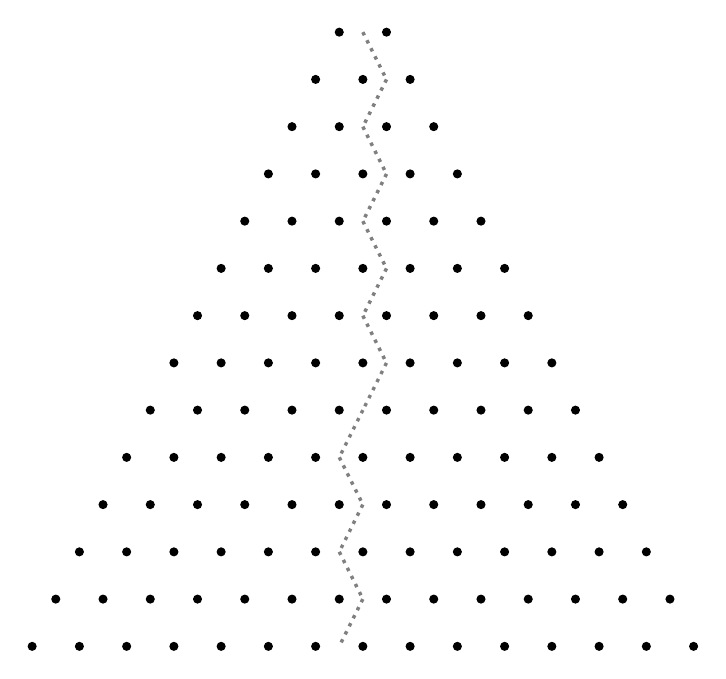
\begin{tikzpicture}%
  \pgfmathsetseed{1}
  \pgfmathsetmacro{\scale}{0.6}
  \pgfmathsetmacro{\x}{0.5*\scale}
  \newcounter{count}\setcounter{count}{0}
  \foreach \row in {2,...,15} {
    \foreach \col in {1,...,\row} {
      \coordinate (pos) at (-\row/2*\scale+\col*\scale,-\row*\scale);
      \node[circle,draw,minimum size=1mm,inner sep=0,fill] at (pos) {};
    }
    \coordinate (a) at (0.5*\value{count}*\scale+0.5*\scale, -\row*\scale);
    \pgfmathparse{rnd}
    \ifdim\pgfmathresult pt > 0.5 pt
    \addtocounter{count}{1}
    \else
    \addtocounter{count}{-1}
    \fi;
    \coordinate (b) at
    (0.5*\value{count}*\scale+0.5*\scale, -\row*\scale-\scale);
    \ifnum\row < 15\draw[color=gray,dotted,line width=1.25pt] (a)--(b)\else\fi;
  }
\end{tikzpicture}
}{
    \caption{Rappresentazione schematica di una macchina di Galton con
      $14$ livelli. La linea spezzata rappresenta una delle possibili
      traiettorie di una pallina lasciata cadere dalla sommità, sotto
      l'ipotesi che ad ogni livello la probabilità di deviare verso destra
      e quella di deviare verso sinistra siano entrambe $\nicefrac{1}{2}$.}
    \label{fig:galton_box}
  }
\end{figure}

A questo punto vi starete chiedendo cosa c'entra tutto questo con i calcolatori
e le sequenze di numeri casuali. Beh\ldots si tratta di un altro esempio di un
sistema che può essere simulato e studiato nel dettaglio con un calcolatore
attraverso l'ausilio di un generatore di numeri casuali. E, a pensarci meglio,
la simulazione si può fare utilizzando lo stesso generatore casuale di
numeri distribuiti uniformemente tra $0$ ed $1$ che abbiamo utilizzato prima:
ad ogni livello possiamo estrarre un numero $r$ tra $0$ e $1$ e dire che se
$r \leq \nicefrac{1}{2}$ ci spostiamo verso sinistra, mentre se
$r > \nicefrac{1}{2}$, allora ci spostiamo a destra. La cosa interessante è
che, nella nostra simulazione, possiamo seguire la pallina dall'inizio alla
fine, proprio come faremmo nella realtà. Possiamo registrare, per ogni
realizzazione del nostro esperimento, non solo il punto di arrivo, ma anche
tutte le posizioni intermedie, che forniscono un quadro dettagliato del nostro
\emph{evento} elementare. In altre parole, ad una qualsiasi domanda che
possiamo pensare di porci a proposito di una macchina di Galton reale, possiamo
dare una risposta con un semplice programma al calcolatore. Il passo da questo
semplice problema di carattere ricreativo alla modellizzazione del moto di
una molecola in un gas o di una particella carica nella materia non è poi
così lungo\footnote{Se volete un esempio più vicino alla vita di tutti
  i giorni pensate al vostro videogioco preferito. Come pensate che faccia
  il calcolatore a generare la varietà imprevedibile di situazioni che lo
  rende interessante?}.

\begin{snippet}[htb!]
  \bigskip % This is ugly and should be taken care of automagically.
  \hstack[0.65]{\begin{Verbatim}[label=\makebox{\href{https://github.com/unipi-physics-labs/lab1-notes/tree/main/snippy/galton_box.py}{https://github.com/.../galton\_box.py}},commandchars=\\\{\}]
\PY{k+kn}{import}\PY{+w}{ }\PY{n+nn}{random}
\PY{n}{random}\PY{o}{.}\PY{n}{seed}\PY{p}{(}\PY{l+m+mi}{1}\PY{p}{)}

\PY{c+c1}{\PYZsh{} Setup the simulation.}
\PY{n}{pos} \PY{o}{=} \PY{l+m+mf}{0.0}
\PY{n}{step} \PY{o}{=} \PY{l+m+mf}{1.0}
\PY{n}{path} \PY{o}{=} \PY{p}{[}\PY{n}{pos}\PY{p}{]}
\PY{c+c1}{\PYZsh{} Loop through the Galton box.}
\PY{k}{for} \PY{n}{i} \PY{o+ow}{in} \PY{n+nb}{range}\PY{p}{(}\PY{l+m+mi}{10}\PY{p}{)}\PY{p}{:}
    \PY{n}{r} \PY{o}{=} \PY{n}{random}\PY{o}{.}\PY{n}{uniform}\PY{p}{(}\PY{l+m+mf}{0.0}\PY{p}{,} \PY{l+m+mf}{1.0}\PY{p}{)}
    \PY{k}{if} \PY{n}{r} \PY{o}{\PYZlt{}}\PY{o}{=} \PY{l+m+mf}{0.5}\PY{p}{:}
        \PY{n}{pos} \PY{o}{=} \PY{n}{pos} \PY{o}{\PYZhy{}} \PY{n}{step}
    \PY{k}{else}\PY{p}{:}
        \PY{n}{pos} \PY{o}{=} \PY{n}{pos} \PY{o}{+} \PY{n}{step}
    \PY{n}{path}\PY{o}{.}\PY{n}{append}\PY{p}{(}\PY{n}{pos}\PY{p}{)}
\PY{c+c1}{\PYZsh{} Print the actual path.}
\PY{n+nb}{print}\PY{p}{(}\PY{n}{path}\PY{p}{)}

[Output]
[0.0, -1.0, 0.0, 1.0, 0.0, -1.0, -2.0, -1.0, 0.0, -1.0, -2.0]
\end{Verbatim}
}{
    \caption{Codice per la simulazione di una semplice macchina di Galton
      (in questo caso a $10$ livelli) che utilizza internamente un generatore
      casuale di numeri reali distribuiti uniformemente tra $0$ ed $1$.
    }
    \label{snip:galton_box}
  }
\end{snippet}


\section{Che cosa è un "numero casuale"?}

Abbiamo visto attraverso due esempi concreti che un generatore di numeri
casuali, se usato opportunamente, può essere uno strumento utile per la
modellizzazione e lo studio di sistemi reali in cui le fluttuazioni casuali
giocano un qualche ruolo. (E, a questo punto, dovrebbe essere chiaro anche il
collegamento tra il "Monte Carlo" nel titolo di questo capitolo e l'argomento
del capitolo stesso.) Adesso si tratta di fare un passo indietro e chiedersi
cosa sia un numero casuale e come si possano generare numeri casuali utilizzando
un calcolatore.

\`E un numero casuale il $3$? Ed il $5$? \`E ovvio che entrambe queste domande
sono prive di senso. Un numero è solo un numero e, di per sé, non è né
casuale né non-casuale. Quello di casualità (o \emph{randomicità}, per
usare un orrendo neologismo che va di moda di questi tempi) è un concetto non
banale da definire con precisione, ma la prima cosa importante da dire è che
esso si applica solo alle \emph{sequenze} di numeri---e non ai numeri singoli.
E allora: cosa possiamo dire della sequenza di cifre decimali
\begin{align*}
  S_1 = 6,~9,~0,~7,~6,~2,~1,~4,~6,~2,~2,~3,~1,~0,~2,~8,~8,~8,~2,~0,~8,~6,~4,~
  8,~5,~9,~9,~2,~8,~3?
\end{align*}
\`E sufficientemente casuale oppure no? E ancora: vi è qualche differenza di
carattere fondamentale (e se sì quale) tra $S_1$ e le due sequenze alternative
\begin{align*}
  S_2 &= 0,~0,~0,~0,~0,~0,~0,~0,~0,~0,~0,~0,~0,~0,~0,~0,~0,~0,~0,~0,~0,~0,~0,~
  0,~0,~0,~0,~0,~0,~0\\
  S_3 &= 0,~1,~2,~3,~4,~5,~6,~7,~8,~9,~0,~1,~2,~3,~4,~5,~6,~7,~8,~9,~0,~1,~2,~
  3,~4,~5,~6,~7,~8,~9?
\end{align*}
Non abbiamo ancora risposto alla domanda con cui abbiamo aperto questa sezione,
ma le sequenze $S_2$ ed $S_3$ non hanno proprio l'apparenza di essere casuali.
$S_2$ contiene solo al cifra $0$ e $S_3$ è la mera ripetizione delle $10$
cifre di partenza, in ordine crescente. $S_1$, invece, non sembra avere niente
che non vada---ed è chiaro che ci serve qualche strumento più sofisticato
per prendere una decisione a proposito del suo livello di casualità.
Eppure, se ci pensiamo meglio, non dovremmo assumere che, in una situazione
veramente casuale, tutte le sequenze di cifre decimali di lunghezza $30$
dovrebbero essere in un qualche senso equiprobabili? Se scegliamo una sequenza
a caso, non dovremmo avere la stessa probabilità di estrarre $S_1$, $S_2$ ed
$S_3$? E allora qual è la differenza fondamentale tra $S_1$ da una parte e
$S_2$ ed $S_3$ dall'altra? Cosa è che ci fa percepire la prima come
potenzialmente casuale e le altre due come decisamente non casuali?
Se un generatore di numeri \foreign{random} ci fornisse $S_3$ come prima
sequenza, saremmo tentati di mettere in dubbio la sua bontà? E, se sì,
perché?

Tutte queste domande sono perfettamente lecite, e mettono in luce alcune
proprietà contro-intuitive del concetto di randomicità---che sono anche
quelle che rendono difficoltosa la sua definizione. La cosa che rende $S_2$ ed
$S_3$ diverse da $S_1$ ai nostri occhi, è il fatto che esse sono
caratterizzate da una struttura ben definita (un \foreign{pattern}) che è
facile da identificare a prima vista. Possiamo descrivere $S_2$ come
"una sequenza di $30$ zeri" e $S_2$ come "tre ripetizioni della sequenza
$0,~1,~2,~3,~4,~5,~6,~7,~8,~9$", mentre è difficile trovare una descrizione
altrettanto concisa di $S_1$. E allora: è vero che, in una situazione
realmente casuale $S_1$, $S_2$ ed $S_3$ sono equiprobabili, ma è anche vero
che ci sono relativamente poche sequenze con \foreign{pattern} così chiari come
in $S_2$ ed $S_3$, immerse in un oceano di sequenze \emph{anonime} come $S_1$.
\`E proprio questo che rende in un qualche senso $S_2$ ed $S_3$ speciali ai
nostri occhi.

Il concetto di \foreign{pattern} è fondamentale in questo contesto, ma dobbiamo
stare attenti a non enfatizzarlo eccessivamente come unico criterio per
decidere se una data sequenza ha buone proprietà di randomicità oppure no.
L'occhio umano è estremamente efficace nell'identificare strutture e
ripetizioni nelle cose, e lasciando libero sfogo a questa nostra capacità si
corre il rischio di eccedere. Guardiamo per un attimo $S_1$ con attenzione, ad
esempio. Ci sono due coppie di cifre che si ripetono ($2,~2$ e $9,~9$) e
addirittura una tripletta ($8,~8,~8$)! Questo vuol dire che in fondo nemmeno
$S_1$ è una sequenza casuale? Beh, se ci pensiamo un attimo la probabilità
di avere una coppia di cifre decimali identiche in successione, assumendo
che esse siano scelte a caso, è $\nicefrac{1}{10}$ e la probabilità di avere
una tripletta è $\nicefrac{1}{100}$, per cui trovare due coppie ed una
tripletta in una sequenza di $30$~cifre non deve sorprenderci. Anzi: se
avessimo una sequenza di $1000$ cifre senza nemmeno una ripetizione potremmo
dire con buona probabilità che essa non è casuale!

Abbiamo insistito abbastanza sul tema ed è tempo di passare oltre. Abbiamo
capito che ci sono alcune proprietà che una sequenza di numeri deve
possedere per poter essere definita casuale. La più ovvia è
l'equidistribuzione (cioè il fatto che le diverse cifre debbono apparire
in media con la stessa frequenza), ma chiaramente essa non è
sufficiente---$S_3$ è equidistribuita ma chiaramente non casuale.
Corrispondentemente esistono svariati test specifici ideati per verificare
la casualità di una sequenza, basati ad esempio sulla distribuzione delle
ripetizioni di cifre (e.g., coppie o triplette) o sulla distanza tra due
occorrenze consecutive della stessa cifra. Si rimanda il lettore a~\cite{taocp2}
per una trattazione approfondita della materia. Per quel che ci riguarda
adotteremo un approccio puramente empirico e diremo che una sequenza è casuale
se, indipendentemente da come essa è stata ottenuta, ha le buone proprietà
cui abbiamo sommariamente accennato (o, equivalentemente, supera tutti i test
rilevanti).


\subsection{Generatori casuali e pseudo-casuali}

Esistono due approcci fondamentalmente diversi per la generazione di
sequenze casuali. Il primo, che è per molti versi il più naturale (ed è
anche il primo in senso storico) si basa sull'idea di utilizzare fenomeni
naturali intrinsecamente casuali---come ad esempio il rumore termico su una
resistenza elettrica o il decadimento di un campione radioattivo. Un generatore
di questo tipo si dice \foreign{true random number generator} (TRNG), ed il
servizio offerto da \url{https://www.random.org/} è un esempio moderno
interessante in cui l'elemento di casualità è il rumore atmosferico.
Vale sicuramente il tempo di un'occhiata veloce.

Dall'altra parte esistono generatori \emph{pseudo-casuali}---che in inglese si
dicono \foreign{pseudo-random number generator} o PRNG---che utilizzano algoritmi
basati su formule matematiche oppure tabelle precompilate per produrre sequenze
di numeri completamente predeterminate che si comportano come se fossero
casuali. Questo può sembrare sorprendente a prima vista: come è possibile
che una sequenza predeterminata sia casuale? Beh, dobbiamo semplicemente
ricordare cosa abbiamo detto alla fine della sezione precedente, e cioè che
giudichiamo una sequenza dalla sue proprietà e non da come è stata
generata. Se una sequenza supera i test di randomicità, allora è casuale
per definizione. Vedremo alcuni esempi concreti nella prossima sezione.

Se dovessimo confrontare sommariamente le proprietà generali dei generatori
casuali e pseudo-casuali diremmo essenzialmente tre cose:
\begin{itemize}
\item I generatori pseudo-casuali sono deterministici, mentre quelli casuali
  sono non deterministici. Nel primo caso la sequenza è univocamente
  determinata dal valore iniziale---e dunque prevedibile e \emph{riproducibile}.
  In pratica la riproducibilità è una proprietà utile perché, come
  vedremo, ci permette di realizzare simulazioni in condizioni controllate.
\item I generatori pseudo-casuali sono periodici, mentre quelli casuali sono
  aperiodici. La periodicità non è un problema in pratica a patto che il
  periodo sia abbastanza lungo. (Per completezza: il generatore pseudo-casuale
  della libreria standard di \python\ ha un periodo $2^{19937} - 1 > 10^{6000}$
  e ci sono meno di $10^{27}$ nanosecondi nell'età dell'Universo, per cui
  la possibilità di esaurire la sequenza è abbastanza remota.)
\item I generatori pseudo-casuali possono essere molto efficienti (in termini
  di numero di cifre prodotte nell'unità di tempo), mentre quelli casuali
  tendono ad essere comparativamente più lenti.
\end{itemize}

Non sorprenderà allora se i generatori pseudo-casuali sono quelli di gran
lunga più utilizzati per applicazioni di modellizzazione e simulazione.
Ma se avete bisogno di generare un numero casuale per l'estrazione di una
lotteria e volete assicurarvi che nessuno possa barare, allora è consigliabile
utilizzare un vero generatore casuale!


\section{La meccanica dei numeri casuali: la ruota della fortuna}

Una delle prime descrizioni dell'utilizzo di dadi per la generazione di numeri
casuali a scopo scientifico risale al 1890 ed è dovuta a Galton~\cite{galton_dice}.
Tra i vari dispositivi meccanici storicamente utilizzati allo scopo, però, in
questa sezione ci soffermiamo su uno che ha una somiglianza sorprendente con
i moderni generatori di numeri pseudo-casuali: la \emph{ruota della fortuna}.

\begin{figure}[htb!]
  \autohstack{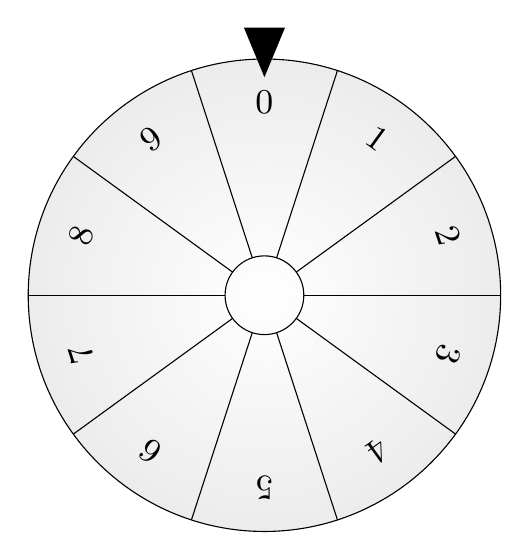
\begin{tikzpicture}
  \usetikzlibrary{shapes.geometric}
  \node at (0, 0) {};

  \pgfmathsetmacro{\radius}{3.}
  \pgfmathsetmacro{\innerradius}{0.5}
  \pgfmathsetmacro{\labelradius}{2.45}
  % adding a subtle gray tone to add a bit of "personality"
  \shade[shading=radial, inner color=white, outer color=gray!15] (0,0) circle (\radius);
  \draw (0,0) circle (\radius);
  \draw (0,0) circle (\innerradius);
  % main lines
  \foreach \x in {0, 36,...,359} \draw (\x:\innerradius) -- (\x:\radius);
  % labels and longer lines at every 10 degrees
  \foreach \x in {0,...,9}
  {
    \node[scale=1.4, rotate=\x*-36] at (360-\x*36+90:\labelradius) {{\small\x}};
    %\draw (\x:\tendegrad) -- (\x:\radius);
  };
  \node[isosceles triangle, draw, fill=black, minimum size=0.5cm, rotate=270] (T) at (0,\radius+0.25){};
\end{tikzpicture}
}{
    \caption{Semplice schema della ruota della fortuna come generatore di numeri
      casuali da $0$ a $9$. Se la velocità iniziale $\omega_0$ è abbastanza grande,
      l'incertezza su $\omega_0$ si accumula ad ogni giro e la posizione finale
      è essenzialmente indeterminata.}
    \label{fig:ruota_fortuna}
  }
\end{figure}

Il nostro modello meccanico della ruota della fortuna è semplicissimo: un
disco messo in rotazione con velocità angolare iniziale $\omega_0$ che rallenta
con un'accelerazione angolare $\alpha$ (che per semplicità consideriamo
nota con precisione infinita, indipendente dalla velocità e costante nel tempo):
\begin{align*}
  \omega(t) = \omega_0 - \alpha t.
\end{align*}
Il tempo $t_0$ a cui la ruota si arresta e l'angolo totale percorso (assumendo che
il disco fosse inizialmente nella posizione $\theta = 0$) si calcolano
facilmente come
\begin{align*}
  t_f = \frac{\omega_0}{\alpha} \quad \text{e dunque} \quad
  \theta_f = \theta(t_f) = \omega_0 t_f - \frac{1}{2}\alpha t_f^2 =
  \frac{\omega_0^2}{2\alpha}.
\end{align*}

Se adesso assumiamo, come è naturale, di non controllare perfettamente la
velocità iniziale---se cioè, nel nostro linguaggio, $\omega_0$ è affetto
da un'incertezza $\sigma_{\omega_0}$---calcolare come questo si ripercuota
sull'angolo totale percorso è un banale esercizio di propagazione dell'errore:
\begin{align*}
  \sigma_{\theta_f} = \frac{\omega_0 \sigma_{\omega_0}}{\alpha} \quad \text{ovvero} \quad
  \frac{\sigma_{\theta_f}}{\theta_f} = 2\frac{\sigma_{\omega_0}}{\omega_0}.
\end{align*}
In altre parole, e giusto per fissare le idee, se controlliamo $\omega_0$ al
$5\%$ (che non è male, visto che azioniamo la ruota manualmente), controlliamo
$\theta_f$ al $10\%$. Ora: il punto fondamentale è che, al termine di ogni giro,
la ruota torna al punto di partenza---a noi non interessa $\theta_f$, ma
$\theta_f~\text{mod}~2\pi$. Equivalentemente, il numero totale di giri percorsi e
l'incertezza associata si scrivono come
\begin{align}\label{eq:ruota_fortuna}
  n = \frac{\theta_f}{2\pi} \quad \text{da cui} \quad
  \frac{\sigma_n}{n} = \frac{\sigma_{\theta_f}}{\theta_f} = 2\frac{\sigma_{\omega_0}}{\omega_0}
  \quad \text{e ancora} \quad \sigma_n = 2n \frac{\sigma_{\omega_0}}{\omega_0}.
\end{align}
Ma quando $\sigma_n \geq 1$ (cioè quando l'incertezza sul numero totale di giri
diventa dell'ordine dell'unità) l'esito diventa essenzialmente indeterminato;
e se $\omega_0$ è noto al $5\%$, $10$ giri sono sufficienti perché ciò accada.
Non c'è molto da aggiungere: la~\eqref{eq:ruota_fortuna} descrive il funzionamento
della ruota della fortuna come generatore di numeri casuali, ed il segreto è
l'aritmetica modulare che vedremo più in dettaglio nella prossima sezione.


\section{Digressione: l'aritmetica modulare}

L'operazione \emph{modulo} non è altro che il resto della divisione intera
tra due numeri---una cosa semplicissima ed apparentemente innocua. Ad esempio
\begin{align*}
  29~\text{mod}~7 = 1 \quad \text{poiché} \quad 29 = 7 \times 4 + 1.
\end{align*}
Eppure l'aritmetica modulare è materia estremamente interessante, e rilevante
(tra le altre cose) per l'argomento di questo capitolo. Vediamo un esempio
concreto: fissati due numeri interi positivi $m$ e $p$, con $p < m$, per
qualsiasi numero intero $k$ sappiamo calcolare banalmente la quantità
\begin{align*}
  0 \leq g = k^p~\text{mod}~m \leq (m - 1)
\end{align*}
Ora, se proviamo a farlo, come mostrato nel frammento~\ref{snip:modulo},
vediamo subito che i risultati sono potenzialmente interessanti. Mentre
$k$ assume tutti i valori da $0$ a $m - 1$ (in quest'ordine), la lista
dei risultati esaurisce la lista degli $m$ valori di $k$, ma in un ordine che
pare aver poco a che vedere con quello di partenza. In un qualche senso abbiamo
riordinato la lista dei primi $m - 1$ interi positivi in modo che appare
casuale. Quello che accade è abbastanza chiaro: al crescere di $k$ si tende
ad avere $k^p \gg m$ ed il risultato del modulo tende ad essere una funzione
discontinua di $k$. L'equivalente meccanico del processo è, per certi
aspetti, la lancetta di un orologio che noi facciamo avanzare a scatti sempre
più grandi. Quando uno scatto corrisponde a molti giri completi, allora la
posizione in cui essa si ferma diviene essenzialmente indeterminata---un po'
come in certi giochi da tavolo (avete presente il gioco della bottiglia?).

\begin{snippet}[htb!]
  \bigskip % This is ugly and should be taken care of automagically.
  \hstack[0.52]{\begin{Verbatim}[label=\makebox{\href{https://github.com/unipi-physics-labs/statnotes/tree/main/snippy/modulo.py}{https://github.com/.../modulo.py}},commandchars=\\\{\}]
\PY{c+c1}{\PYZsh{} Define m and p, and initialize an empty list.}
\PY{n}{m} \PY{o}{=} \PY{l+m+mi}{11}
\PY{n}{p} \PY{o}{=} \PY{l+m+mi}{7}
\PY{n}{sequence} \PY{o}{=} \PY{p}{[}\PY{p}{]}
\PY{c+c1}{\PYZsh{} Calculate k\PYZca{}p mod m for all positive k \PYZlt{} m.}
\PY{c+c1}{\PYZsh{} Note ** is the power and \PYZpc{} the modulo operator.}
\PY{k}{for} \PY{n}{k} \PY{o+ow}{in} \PY{n+nb}{range}\PY{p}{(}\PY{n}{m}\PY{p}{)}\PY{p}{:}
    \PY{n}{sequence}\PY{o}{.}\PY{n}{append}\PY{p}{(}\PY{n}{k}\PY{o}{*}\PY{o}{*}\PY{n}{p} \PY{o}{\PYZpc{}} \PY{n}{m}\PY{p}{)}
\PY{c+c1}{\PYZsh{} Print the sequence.}
\PY{n+nb}{print}\PY{p}{(}\PY{n}{sequence}\PY{p}{)}

[Output]
[0, 1, 7, 9, 5, 3, 8, 6, 2, 4, 10]
\end{Verbatim}
}{
    \caption{Esempio di calcolo di $k^p~\text{mod}~m$ per $m = 11$, $p = 7$
      e $0 \leq k < m$. Si sarebbe tentati di dire che l'effetto è quello di
      riordinare la lista di partenza $[0\ldots m- 1]$ in modo
      apparentemente casuale. (L'effetto qui non è eclatante, ma divertitevi
      a modificare il programma e ripetere l'esercizio con due numeri primi $m$
      e $p$ ragionevolmente grandi).
    }
    \label{snip:modulo}
  }
\end{snippet}


\subsection{Il logaritmo discreto}

Il problema è anche più interessante di così. Adesso possiamo porci una
domanda leggermente diversa, ovverosia: dato un intero positivo $m$ e due interi
$0 \leq p,~g < m$, come possiamo calcolare il valore di $k$ per cui
\begin{align}\label{eq:logaritmo_discreto}
  p^k~\text{mod}~m = g?
\end{align}
Il lettore non avrà mancato di notare l'analogia con il logaritmo ordinario
nel campo dei numeri reali, ed in effetti la soluzione $k$
della~\eqref{eq:logaritmo_discreto} si dice solitamente logaritmo discreto di
$g$ in base $b$ (modulo $m$).

\pgffigone{logaritmo_discreto}{
  Illustrazione del problema del logaritmo discreto per $m = 71$ e $p = 11$.
  Al variare di $k = 0\ldots m - 1$ i valori di $p^k~\text{mod}~m$ variano
  in modo estremamente irregolare, il che rende difficile calcolare la
  soluzione di $p^k~\text{mod}~m = g$, se non provando tutti i $k$.
}

Il problema del logaritmo discreto è importante in crittografia
perché è considerato di difficile soluzione---almeno quando si tratta di
numeri grandi. La figura~\ref{fig:logaritmo_discreto} illustra quanto
$p^k~\text{mod}~m$ vari in modo irregolare al variare di $k$, per cui è
estremamente difficile immaginare una strategia generale per calcolare il
logaritmo discreto che non sia la forza bruta (cioè provare tutti i valori
di $k$ uno dopo l'altro fino a quando non troviamo la soluzione).


\section{Sequenze pseudo-casuali}

Uno dei primi schemi per la generazione di sequenze pseudo-casuali con un
calcolatore è dovuta a John Von Neumann e risale alla metà degli
anni '40 del '900. L'algoritmo di base è molto semplice: partiamo da un
numero intero $X_0$ di $m$ cifre (che chiamiamo \emph{seme} o \foreign{seed}), e
definiamo una successione per ricorrenza con la prescrizione che ad ogni passo
prendiamo le $m$ cifre centrali del quadrato dell'elemento
precedente---ovverosia, in rappresentazione decimale:
\begin{align}\label{eq:middle_square}
  X_{n + 1} = (X_n^2 / 10^{\frac{m}{2}})~\text{mod}~10^m.
\end{align}
Il metodo di Von Neumann è generalmente noto con il nome di \foreign{middle square},
ed è più complicato a spiegarsi in maniera descrittiva che non con un esempio---cosa
che facciamo prontamente nella tabella~\ref{tab:middle_square}.

\begin{table}[htb]
  \tablehstack{
    \begin{tabular}{lllll}
      \hline
      $n$ & $X_n$ & $X_n^2$ & $X_n^2 / 10^{\frac{m}{2}}$ & $X_{n + 1}$\\
      \hline
      \hline
      $0$ & $3333$ & $11\underline{1088}89$ & $111088$ & $1088$\\
      $1$ & $1088$ & $01\underline{1837}44$ & $011837$ & $1837$\\
      $2$ & $1837$ & $03\underline{3745}69$ & $033745$ & $3745$\\
      $3$ & $3745$ & $14\underline{0250}25$ & $140250$ & $0250$\\
      $4$ & $0250$ & $00\underline{0625}00$ & $000625$ & $0625$\\
      $5$ & $0625$ & $00\underline{3906}25$ & $003906$ & $3906$\\
      $6$ & $3906$ & $15\underline{2568}36$ & $152568$ & $2568$\\
      $7$ & $2568$ & $06\underline{5946}24$ & $065946$ & $5946$\\
      $8$ & $5946$ & $35\underline{3549}16$ & $353549$ & $3549$\\
      $9$ & $3549$ & $12\underline{5954}01$ & $125954$ & $5954$\\
      \hline
    \end{tabular}
  }{
    \caption{Illustrazione del metodo \foreign{middle square} per la generazione
      di sequenze pseudo-casuali con $m = 4$ cifre decimali e seme
      iniziale $X_0 = 3333$. (Va da sé che in un calcolatore l'algoritmo
      sarebbe più efficiente se implementato in logica binaria anziché
      decimale.) Nella terza colonna sono sottolineate le $4$
      cifre centrali tra le $8$ che costituiscono il quadrato dell'$n$-simo
      numero nella sequenza, ma per completezza la quarta e la quinta colonna
      mostrano i singoli passi della~\eqref{eq:middle_square}
      separatamente.
    }
    \label{tab:middle_square}
  }
\end{table}

L'idea di base è che le cifre centrali del risultato dell'elevamento al
quadrato dipendono in modo complicato dal numero di partenza e possono essere
considerate come un numero di $m$ cifre essenzialmente scorrelate da esso.
Retrospettivamente possiamo dire che il metodo \foreign{middle square} non
è soddisfacente secondo gli standard moderni, ed il suo interesse è ormai
di carattere prevalentemente storico. Una delle limitazioni maggiori consiste
nella tendenza dell'algoritmo di rimanere intrappolato in cicli di lunghezza
molto breve. Potete verificare, ad esempio, che se scegliamo $2500$ come seme
per il nostro generatore a $4$ cifre, la~\eqref{eq:middle_square} trasforma
$X_0$ in se stesso indefinitamente. Purtuttavia forniamo un'implementazione
utilizzabile del metodo nel frammento~\ref{snip:middle_square}.

\begin{snippet}[htb!]
  \bigskip % This is ugly and should be taken care of automagically.
  \hstack[0.675]{\begin{Verbatim}[label=\makebox{\href{https://github.com/unipi-physics-labs/statnotes/tree/main/snippy/middle_square.py}{https://github.com/.../middle\_square.py}},commandchars=\\\{\}]
\PY{c+c1}{\PYZsh{} Middle\PYZhy{}square random number generator with m = 4.}
\PY{c+c1}{\PYZsh{} Define the seed and print it out.}
\PY{n}{x} \PY{o}{=} \PY{l+m+mi}{3333}
\PY{n}{sequence} \PY{o}{=} \PY{p}{[}\PY{n}{x}\PY{p}{]}
\PY{c+c1}{\PYZsh{} Generate 10 numbers\PYZhy{}\PYZhy{}\PYZhy{}note 10\PYZca{}\PYZob{}m/2\PYZcb{} = 100 and 10\PYZca{}m = 10000.}
\PY{k}{for} \PY{n}{n} \PY{o+ow}{in} \PY{n+nb}{range}\PY{p}{(}\PY{l+m+mi}{10}\PY{p}{)}\PY{p}{:}
    \PY{n}{x} \PY{o}{=} \PY{p}{(}\PY{n}{x}\PY{o}{*}\PY{o}{*}\PY{l+m+mi}{2} \PY{o}{/}\PY{o}{/} \PY{l+m+mi}{100}\PY{p}{)} \PY{o}{\PYZpc{}} \PY{l+m+mi}{10000}
    \PY{n}{sequence}\PY{o}{.}\PY{n}{append}\PY{p}{(}\PY{n}{x}\PY{p}{)}
\PY{c+c1}{\PYZsh{} Print the sequence.}
\PY{n+nb}{print}\PY{p}{(}\PY{n}{sequence}\PY{p}{)}

[Output]
[3333, 1088, 1837, 3745, 250, 625, 3906, 2568, 5946, 3549, 5954]
\end{Verbatim}
}{
    \caption{Possibile implementazione dell'algoritmo \foreign{middle square}
      per la generazione della sequenze di $10$ elementi illustrata in
      tabella~\ref{tab:middle_square}.}
    \label{snip:middle_square}
  }
\end{snippet}


\subsection{Aspetti generali dei generatori pseudo-casuali}

L'algoritmo \foreign{middle square} descritto nella sezione precedente, benché
ormai di scarsa rilevanza pratica per i motivi che abbiamo visto, è
importante perché esemplifica almeno due aspetti fondamentali di molti
generatori pseudo-casuali utilizzati in pratica. Il primo è l'idea
di base di generare ricorsivamente gli elementi (interi) della sequenza
\begin{align}\label{eq:generatore_iterativo}
  X_{n + 1} = f(X_n)
\end{align}
a partire da un seme (o \foreign{seed}) $X_0$ ed utilizzando una funzione
$f: [0,~X_\text{max}] \rightarrow [0,~X_\text{max}]$. (Questa funzione può
essere applicata all'elemento precedente della sequenza o, più in generale
ad una $n$-tupla di elementi.) Il secondo è quello di sfruttare
l'aritmetica modulare per far sì che la sequenza si comporti
\emph{come se fosse casuale}. Torneremo sull'argomento tra un attimo.

Prima di andare avanti soffermiamoci un momento sui due esempi con cui abbiamo
aperto questo capitolo: il calcolo di $\pi$ e la macchina di Galton---in
entrambi i casi abbiamo utilizzato un generatore casuale di numeri reali
compresi tra $0$ ed $1$. Qual è, allora la connessione con
la~\eqref{eq:generatore_iterativo}?
Molto semplicemente, detto $X_\text{max}$ il valore massimo restituito da $f(X)$,
che per esempio è $10^m - 1$ nel generatore~\eqref{eq:middle_square},
possiamo semplicemente dividere $X_n$ per $X_\text{max} + 1$
\begin{align}
  U_n = \frac{X_n}{X_\text{max} + 1}
\end{align}
per ottenere una sequenza $U_n$ di numeri reali tra $0$ ed $1$---o, più
precisamente, nell'intervallo $[0,~1)$. Va da sé che la granularità non
sarà infinita (tecnicamente avremo numeri razionali con precisione
$\nicefrac{1}{X_\text{max}}$), ma questo è irrilevante, perché
l'aritmetica in virgola mobile su un calcolatore è comunque inesatta (come
discusso sommariamente in appendice~\ref{sec:sistema_binario}).

Torniamo alla nostra definizione per ricorrenza. Una conseguenza immediata
della~\eqref{eq:generatore_iterativo} è che il \emph{periodo} della sequenza
sarà necessariamente limitato: avendo a disposizione un numero finito di
interi, ad un certo punto la nostra funzione $f$ trasformerà l'elemento
$n$-esimo in un numero che abbiamo già ottenuto in precedenza e, da quel
punto in poi, la sequenza si ripeterà in un ciclo infinito. Quando questo
accade, la sequenza cessa di comportarsi come se fosse casuale, per cui il
periodo costituisce un limite superiore al numero di elementi che si possono
estrarre utilmente. Tutto ciò non è un problema in pratica se il periodo
è abbastanza lungo, per cui è chiaro che questa è una delle considerazioni
fondamentali nel disegno di un generatore.


\subsection{Lo schema lineare congruenziale}

Lo schema lineare congruenziale (\foreign{linear congruential method}),
proposto all fine degli anni '40 del secolo scorso, è ancora oggi
abbastanza popolare, e lo discutiamo brevemente. La definizione di base è
\begin{align}
  X_{n + 1} = (a X_n + c)~\text{mod}~m
\end{align}
in cui il moltiplicatore $a$, l'incremento $c$ ed il modulo $m$ sono
tre numeri fissi opportunamente scelti. (Ovviamente abbiamo anche bisogno di
un seme $X_0$ per definire univocamente la sequenza---e diversi valori del
seme danno origine a diverse sequenze.) Il fatto di prendere il risultato
dell'operazione tra parentesi modulo $m$ implica che il massimo numero
ottenibile $X_\text{max} = m - 1$ e che il periodo massimo ottenibile è
esattamente $m$. In generale non è garantito che, per una terna arbitraria
di valori $a$, $c$ ed $m$, la sequenza abbia periodo massimo, ma esistono
condizioni ben definite perché questo accada~\cite{taocp2}.

\begin{snippet}[htb!]
  \bigskip % This is ugly and should be taken care of automagically.
  \hstack[0.6]{\begin{Verbatim}[label=\makebox{\href{https://github.com/unipi-physics-labs/statnotes/tree/main/snippy/lcg1.py}{https://github.com/.../lcg1.py}},commandchars=\\\{\}]
\PY{c+c1}{\PYZsh{} Toy two\PYZhy{}digit (0\PYZhy{}\PYZhy{}99) linear congruential generator.}
\PY{n}{a} \PY{o}{=} \PY{l+m+mi}{11}
\PY{n}{c} \PY{o}{=} \PY{l+m+mi}{3}
\PY{n}{m} \PY{o}{=} \PY{l+m+mi}{73}
\PY{n}{x} \PY{o}{=} \PY{l+m+mi}{81}

\PY{c+c1}{\PYZsh{} Generate 10 numbers.}
\PY{n}{sequence} \PY{o}{=} \PY{p}{[}\PY{p}{]}
\PY{k}{for} \PY{n}{i} \PY{o+ow}{in} \PY{n+nb}{range}\PY{p}{(}\PY{l+m+mi}{10}\PY{p}{)}\PY{p}{:}
    \PY{n}{x} \PY{o}{=} \PY{p}{(}\PY{n}{a} \PY{o}{*} \PY{n}{x} \PY{o}{+} \PY{n}{c}\PY{p}{)} \PY{o}{\PYZpc{}} \PY{n}{m}
    \PY{n}{sequence}\PY{o}{.}\PY{n}{append}\PY{p}{(}\PY{n}{x}\PY{p}{)}

\PY{n+nb}{print}\PY{p}{(}\PY{n}{sequence}\PY{p}{)}

[Output]
[18, 55, 24, 48, 20, 4, 47, 9, 29, 30]
\end{Verbatim}
}{
    \caption{Esempio di implementazione di un generatore lineare congruenziale
      giocattolo di numeri interi a due cifre decimali con periodo massimo
      ($100$).}
    \label{snip:lcg1}
  }
\end{snippet}

Per completezza, il frammento~\ref{snip:lcg1} implementa un generatore
\emph{giocattolo} di numeri interi a due cifre decimali utilizzando lo schema
lineare congruenziale. Notiamo, per inciso, che il suo periodo è il massimo
possibile ($100$) per un generatore a due cifre decimali.

\begin{snippet}[htb!]
  \bigskip % This is ugly and should be taken care of automagically.
  \hstack[0.6]{\begin{Verbatim}[label=\makebox{\href{https://github.com/unipi-physics-labs/statnotes/tree/main/snippy/lcg2.py}{https://github.com/.../lcg2.py}},commandchars=\\\{\}]
\PY{c+c1}{\PYZsh{} Real (i.e., usable) linear congruential generator.}
\PY{n}{a} \PY{o}{=} \PY{l+m+mi}{6364136223846793005}
\PY{n}{c} \PY{o}{=} \PY{l+m+mi}{1442695040888963407}
\PY{n}{m} \PY{o}{=} \PY{l+m+mi}{2}\PY{o}{*}\PY{o}{*}\PY{l+m+mi}{64}
\PY{n}{x} \PY{o}{=} \PY{l+m+mi}{1}

\PY{c+c1}{\PYZsh{} Generate 10 number between 0 and 1.}
\PY{k}{for} \PY{n}{i} \PY{o+ow}{in} \PY{n+nb}{range}\PY{p}{(}\PY{l+m+mi}{10}\PY{p}{)}\PY{p}{:}
    \PY{n}{x} \PY{o}{=} \PY{p}{(}\PY{n}{a} \PY{o}{*} \PY{n}{x} \PY{o}{+} \PY{n}{c}\PY{p}{)} \PY{o}{\PYZpc{}} \PY{n}{m}
    \PY{n}{u} \PY{o}{=} \PY{n+nb}{float}\PY{p}{(}\PY{n}{x}\PY{p}{)} \PY{o}{/} \PY{p}{(}\PY{n}{m} \PY{o}{\PYZhy{}} \PY{l+m+mi}{1}\PY{p}{)}
    \PY{n+nb}{print}\PY{p}{(}\PY{n}{u}\PY{p}{)}

[Output]
0.42320917087271326
0.5094074428837206
0.6483593939634306
0.38286339050826024
0.795447749253532
0.5005112827950045
0.5539353613127292
0.0654193119742375
0.8397261096476889
0.19844004278856292
\end{Verbatim}
}{
    \caption{Esempio di implementazione di un generatore lineare congruenziale
      di numeri in virgola mobile (equidistribuiti tra $0$ ed $1$) utilizzabile
      in pratica, con periodo $2^{64}$.}
    \label{snip:lcg2}
  }
\end{snippet}

Il frammento~\ref{snip:lcg2}, viceversa, illustra un generatore realistico,
dotato di un periodo di $2^{64} \approx 1.8 \times 10^{19}$. Non è niente in
confronto al generatore di tipo \emph{Mersenne-Twister}~\cite{mersenne_twister}
implementato nella libreria standard di \python\ (che, come abbiamo detto, ha un
periodo di $2^{19937} - 1$) ma potrebbe sicuramente essere utilizzato in
situazioni non estremamente complesse. (Al solito: se volete utilizzare
numeri pseudo-casuali professionalmente, evitate di re-inventare la ruota ed
utilizzate direttamente \numpy, come illustrato nella sezione che segue.)


%\section{Generazione di numeri pseudo-casuali con distribuzione non uniforme}

%A questo punto abbiamo un'idea abbastanza precisa di come si possano generare
%numeri pseudo-casuali distribuiti tra $0$ ed $1$. Il prossimo passo ovvio
%è chiedersi come si possano generare numeri pseudo-casuali con
%distribuzioni diverse.


\summary


\begin{itemize}
  \item I metodi Monte Carlo sono basati sulla generazione di sequenze
  pseudo-casuali di numeri, e costituiscono una delle tecniche fondamentali per
  la simulazione di processi fisici.
  \item Tutti i linguaggi di programmazione---e \python\ non fa eccezione---forniscono
  librerie per la generazione di numeri pseudo-casuali distribuiti secondo
  le più comuni distribuizioni di probabilità.
\end{itemize}
